\documentclass{llncs}

\usepackage{graphicx}
\usepackage{subfig}
\usepackage{xspace}

\newcommand{\ompi}{Open\,MPI\xspace}
\begin{document}

\title{Fault Tolerant Runtime for Open MPI}
\author{Wesley Bland}

\maketitle

\begin{abstract}
  If the MPI library, or any other parallel environment, expects
  non-failed processes to continue their execution despite failures,
  it is necessary that the runtime supporting the parallel execution
  environment becomes resilient to such failures. Such a fault
  tolerant runtime is required to remain capable of providing its
  services, in addition to offering additional services related to
  faults. Thus, runtime environments have a key role to play in
  resilient capabilities of an MPI implementation. In this paper, we
  introduce a minimalistic set of basic services related to fault
  handling, and we present and evaluate a resilient runtime
  environment, adapted from ORTE, the runtime environment of
  \ompi. \end{abstract}

\section{Introduction} \label{sect:introduction}

% Need for fault tolerance
	% Large Machines - Top500
	% Shrinking MTTF - Schroeder and Gibson
Fault tolerance is an increasingly necessary consideration in high
performance computing (HPC). As machine sizes increase past hundreds
of thousands of computing cores\footnote{http://www.top500.org} into
the millions computing resources, the likelihood of failures also
increases. Schroeder and Gibson~\cite{4775906} announced a mean time
between failure (MTBF) on some of the machines at Los Alamos National
Laboratory (LANL) of 8 hours. This work was published in 2007 and the
MTBF of large-scale machines is only expected to shrink as the machine
size grows.
	
% \ompi
	% Short Intro - Citation?
	% Some fault tolerance already
		% Checkpoint / Restart
	% Need resilient runtime
The \ompi Project is an open source MPI-2 implementation that is
developed and maintained by a consortium of academic, research, and
industry partners~\footnote{http://www.open-mpi.org}. It has already
made strides to include some fault tolerance support by developing
checkpoint/restart and message logging frameworks, allowing users to
recover processes that fail by reverting to a previously stored
snapshot of the application. While this method of fault tolerance is
useful for many applications, as the number of processes increases,
the overhead of saving the state of as many as millions of concurrent
processes becomes untenable and other methods of fault tolerance must
be envisioned.

Other approaches, not based on coordinated checkpointing, have been
proposed to tackle this issue, each one addressing the fault at a
different level in the software stack. In Algorithmic Based Fault
Tolerance approaches~\cite{494110}, the surviving processes will
regenerate the data, and continue the computation with substitute
processes; other times (e.g. using uncoordinated checkpointing with
message logging~\cite{mpichv2}), the MPI system itself will start
substitute processes and provide them with the information needed to
ensure the consistency of the recovery. In other situations (e.g. a
Monte-Carlo simulation), failed processes can simply be ignored, and
the computation continue without replacing them or recovering their
data.
% In all these situations, the application and/or the MPI environment
% require that the non-failed processes continue to work.
The common point between these more scalable approaches is that
non-failing processes need to continue participating in the
application, and therefore need support from their managing runtime to
achieve this goal.

To ensure this continued progression, the MPI environment relies on a
runtime system. In this paper, we focus on the first building block
necessary to produce a resilient MPI implementation: a resilient
runtime for MPI. The responsibilities of the runtime system with
respect to resiliency are twofold:

\begin{description}

\item[Fault Detection] Failure detection requires, in many systems, to
  actively probe the reactivity of processes. Since the application
  processes may enter com\-pu\-ta\-tion-intensive phases for an arbitrary
  duration, another level must be responsible to answer these probes,
  serving as witness of activity for remote monitoring processes. In
  most environments, the runtime processes are best suited to
  accomplish this role.

\item[Fault Notification] Once a failure is detected, all processes
  that interact with the failed processes (this is often all processes
  of the system, by closure of the connected relationship as defined
  by the MPI standard) must be eventually notified in order for them
  to take correcting actions. This notification could have happened
  inside the MPI library, but because the runtime system must already
  provide a resilient out-of-band communication mechanism, we consider
  that this is a role that it can better fulfill.

\end{description}

Once the application is notified of failures, it will take corrective
actions. These actions (like starting new processes to replace the
failed ones) may require services from the runtime level to work. Even
if no special corrective actions are necessary, the runtime system
needs to continue providing its basic services (I/O forwarding,
termination and cleaning of the application, out-of-band messaging
system) to the parallel application until its normal termination point
is reached.

In this paper, we present how an MPI runtime system can be made
resilient, to continue providing its services in presence of fail-stop
failures. We evaluate the performance of this runtime system
using ad-hoc applications by comparing it with the performance of a
non-resilient runtime system and through micro-benchmarks in the
presence of different scenarios of faults.

% Outline paper
Section~\ref{sect:related} of this paper will outline previous work in
this field as well as describe the \ompi architecture.
%Section~\ref{sect:motivation} will describe the motivation behind this work. 
Section~\ref{sect:methodology} will present the changes we have
introduced to implement the resilient layer of the runtime system.
Section~\ref{sect:results} will showcase the performance of the work,
and Section~\ref{sect:conclusion} will summarize the work and point to
future research.

\section{Related Work}
\label{sect:related}

Many other groups have worked on fault tolerant runtimes in the past
that each use different methods of fault tolerance. Most of these
runtimes focus on employing checkpoint/restart, but a few also use new
ideas to prevent or recover from process failures.

% Charm++ & Adaptive MPI

Charm++ is an object-oriented parallel programming language developed
at the University of Illinois at
Urbana-Champaine~\cite{Kale93charm++:a}. In addition to message
passing, it also performs load balancing, process migration and other
interesting properties due to the fact that it treats each process as
an individual object, called ``chares'', that can be saved and moved
at any time. This has lead to work which leverages these chares to
provide fault tolerance guarantees~\cite{10.1109/CLUSTR.2004.1392606},
including an MPI implementation which uses Charm++ as its
runtime~\cite{ampiJournal}.

% FT-MPI

FT-MPI extended the MPI semantics provided by the MPI standard to
include fault tolerance. This enabled application developers to adapt
their applications without the need to rewrite them using an entirely
different message passing
system~\cite{Fagg:2000:FFT:648137.746632,Fagg:2004vd}. FT-MPI could
withstand $n-1$ process failures in a job of size $n$. This is similar
to the work being done in this paper as both are designed to recover
from arbitrary fail-stop failures. However, FT-MPI only provides this
semantic to the functions supported by the version 1.2 of the MPI
standard.

% Other MPI runtimes?

% MPI 3 FT Run-Through Stabilization, Process Recovery

The MPI forum in currently in the process of writing the new MPI
specification, MPI 3. Expected in this version of the specification is
language to describe how MPI applications should handle process faults
including both stabilization and recovery of failed processes. This
work is being done publicly and progress can be found on the MPI 3
Fault Tolerance Working Group's
website\footnote{https://svn.mpi-forum.org/trac/mpi-forum-web/wiki/FaultToleranceWikiPage}.

% \ompi architecture (OMPI, ORTE, OPAL)

% Motivation
% \section{Motivation}
% \label{sect:motivation}

% This work was motivated by the need to demonstrate a runtime that
% can quickly recover from a process failure by stabilizing internal
% bookkeeping and communications. The runtime must inform the
% application of the failure and return to normal operation. While
% this particular implementation of that runtime is one example of the
% desired runtime, it is not the only method of writing that runtime.
% This runtime was not written to demonstrate superb performance and
% should not be used a barometer to measure the feasibility of a low
% overhead implementation, though the overhead of this implementation
% will be examined in section~\ref{sect:results} in the interest of a
% complete examination.

% Other implementations are expected to follow this prototype and
% perhaps improve performance or change the method of stabilization.
% This work however, shows that such implementations can exist and
% work should continue to create them. It provides a basic framework
% for MPI implementors to add their own MPI layer on top of the
% runtime without the need for their own runtime system.

\section{A Resilient Runtime}
\label{sect:methodology}

We present in this section how the \ompi Runtime Environment
(ORTE)~\cite{Castain:2008dx} has been modified to become resilient as
an example of the expected changes that need to be undergone on
runtime environments to provide resilient capabilities. We focus first
on how the runtime itself has been made fault tolerant; then on the
additional services that the runtime should provide to its user (the
MPI library or any other parallel environments): Failure Detection and
Notification. The modified runtime is capable of running any MPI
application. However, since the MPI
level does not provide a stabilization interface yet, the MPI
application cannot use the additional services to continue its
execution.

\subsection{Out-Of-Band Message Consistency Using Epochs}
\label{subsect:epochs}
Before implementing process recovery, a way of tracking the status of
processes is necessary. A commonly used method in literature is to add
an epoch to the process naming scheme. The epoch tracks the number of
times a process has failed by incrementing the epoch every time the
{\em Head Node Process} (HNP) is notified of a failure. The runtime
uses this epoch to prevent transient process failure from introducing
unexpected behavior by cutting off a process with an epoch less than
the most recent value from interfering with the other processes. As
each message is processed by the communication library, it is checked
against the most recent known epoch for the originating process. If
the message's epoch is less than the most recently known epoch, the
message is dropped and will need to be retransmitted to the new
version of the previously failed process. This essentially forces a
fail-stop fault model~\cite{FLP85} upon the processes, simplifying error detection
and recovery.
	
\subsection{Fault Handling}
\label{subsect:handling}

Concurrently with the notification of failure throughout the runtime,
the HNP and the ORTE daemons (ORTEDs) also perform fault handling tasks to stabilize
the runtime and allow processes to continue. The most noticeable
portion of the runtime that must be updated is the routing layer. Most
routing layers have some sort of topology that passes messages from
one node to the next rather than all messages being routed through the
HNP. This routing layer must be mended after any of the nodes fails.
One of the most common routing topologies is a tree. When the fault is
detected, the tree must remove the faulty process and create
connections from the failed process's parent to its children. This
must also take into account any subsequent failures so that if
necessary, the routing layer will continue to look upward or downward
in the tree to find the closest living neighbor and prevent any child
from becoming orphan due to a lack of connection to a living parent.

% Failure Detection
\subsection{Failure Detection}
\label{subsect:detection}

Failure detection is accomplished using the existing detectors in
ORTE. The primary detection method is to monitor the status of
communication channels. If a connection fails, the ORTE error handler
begins the process of managing the fault as detailed in
Section~\ref{subsect:handling}. In the future, when an MPI layer will
be placed on top of the runtime, it will need to send errors to the
runtime if it wants the errors to be handled in a consistent way. The
current method of handling failures in MPI is to abort as soon as
possible after detecting an error. By passing the error information to
the runtime rather than acting within the MPI layer, that singular
method of handling faults can be improved and the application may
survive the fault.

% Failure notification
	% ORTEDs notice failures and notify HNP
	% Currently limited to communication failures but any detector can be plugged in
	% ORTEDs react while message is sent to HNP
	% HNP broadcasts failure message to all ORTEDs which tell the application layers
	% Everyone marks the process as dead and continues
	% Hook to notify MPI layer in place
% Messages to dead processes are dropped
	% Application will be notified with process failure notification
% Routing layer removed routes to dead processes
	% Routes around and creates new routes
\subsection{Failure Notification}
When a failure occurs, ORTE quickly attempts to stabilize the runtime
system to allow the surviving processes to continue. The first step in
this process is to notify the HNP. The HNP is responsible for
maintaining the state of the application and notifying all runtime
processes of any changes to which they need to respond. Once the HNP
has received the message from the ORTEDs who detected
the failure, it broadcasts this information to all other daemons.
While some of them might already know about the failure, because they
detected it via the direct connections between daemons, by including
the epoch of the failed process they can prevent duplicate or
out-of-order handling of the faults. At this point, the runtime would
notify the MPI layer of the error, therefore allowing the MPI
processes themselves to decide how the parallel application will
react to the fault.
% A group is implementing MPI level fault tolerance based on the work
% of the MPI Forum Fault Tolerance Working Group and their work will
% be available soon for testing. In the meantime, applications that
% use the ORTE layer directly can register a callback function so they
% will be notified directly when a process fails and handle it
% application level.

% Added epoch to process name
	% Prevents send/receive from already dead processes
	% Helps bookkeeping when tracking process status

\section{Results}
\label{sect:results}

% Can withstand failure in any process other than HNP

0

To test our implementation of the fault tolerant runtime, we use a
simple ring and token test. Rank 0 generates a group of tokens and
periodically sends one around the ring. As each rank receives the
token, it immediately passes it to the next rank in the ring. After a
parameterized number of tokens passes a rank it simulates a process
failure. We use this test with a variety of failure patterns to
demonstrate the performance impact of multiple failures on the
runtime. Our runtime can withstand a failure from any process at any
time other than the HNP. This is an acceptable constraint
however because while the probability of losing \emph{any}
node is high, the probability of losing a \emph{specific}
node is relatively low. This is increasingly true as individual
machine reliability improves. Because there are currently no MPI
semantics for fault tolerance, we can only use runtime level
communication and process management. Our tests were run using 64
nodes on Grid5000.\footnote{Experiments presented in this paper were
  carried out using the Grid'5000 experimental testbed, being
  developed under the INRIA ALADDIN development action with support
  from CNRS, RENATER and several Universities as well as other funding
  bodies (see https://www.grid5000.fr)} Rank 0 generated 4000 tokens
to be sent around the ring. After completing a circuit of the ring,
rank 0 recaptures the tokens and gather data about the round trip time
and number of hops.

The ring token test has been written as an ORTE application. After it
initializes the ORTE subsystem, each rank reads a scenario file, that
defines how failures will happen (if any), and registers a fault
handler that will take statistics on the time of failures
notifications. Then, the root process (process of \texttt{vpid} 0)
starts sending the tokens, and other processes forward them according
to the ring algorithm. After the scenario has been completed, each
process still alive finalizes the ORTE subsystem, and prints
statistics of the run.

% Compare ring/token test FF vs. failure

In Figure~\ref{fig:onebyone}, processes fail one at a time in evenly
spaced intervals until only 2 processes remain. As each process fails,
the round trip time decreases linearly. This is the expected behavior
as each token must traverse fewer ranks until it reaches rank 0
again. The number of hops decreases slowly as each process fails, but
the round trip time with failures actually decreases at a greater rate
temporarily. This is because the buffers at the first few ranks become
full at the beginning of the run when the tokens are still being
generated. As the buffers clear the first few ranks, the round trip
time stabilizes into a linear speedup.

In Figure~\ref{fig:burst}, processes fail in groups of two. This shows
that the runtime can withstand larger groups of processes failing at
roughly the same time. This would simulate a two processor node
failing at once. The gaps in the graph show the points at which some
tokens are lost. This is expected as the application makes no attempt
to recover or regenerate tokens temporarily hosted by failed
processes, and simply continues to run with whatever tokens return
back to rank 0.

\begin{figure}[t]
  \centering
  \subfloat[\small N/2 Processes Failing at Midpoint]{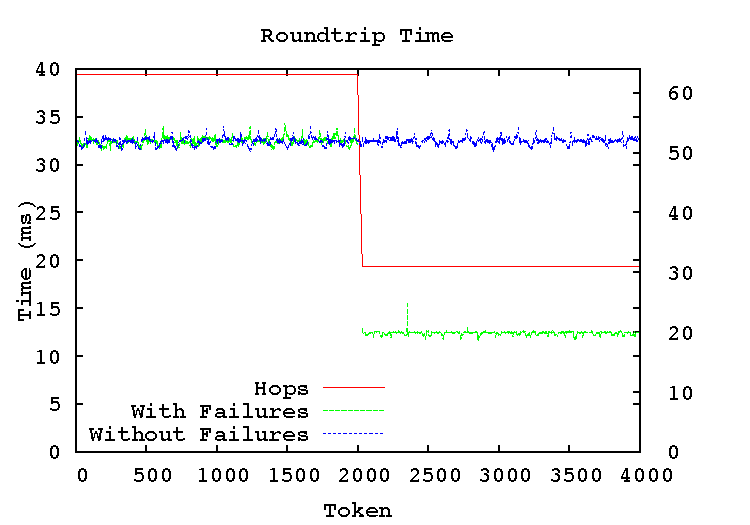
\includegraphics[scale=0.48]{major.pdf}\label{fig:major}}
  \subfloat[\small N-2 Processes Failing at Midpoint]{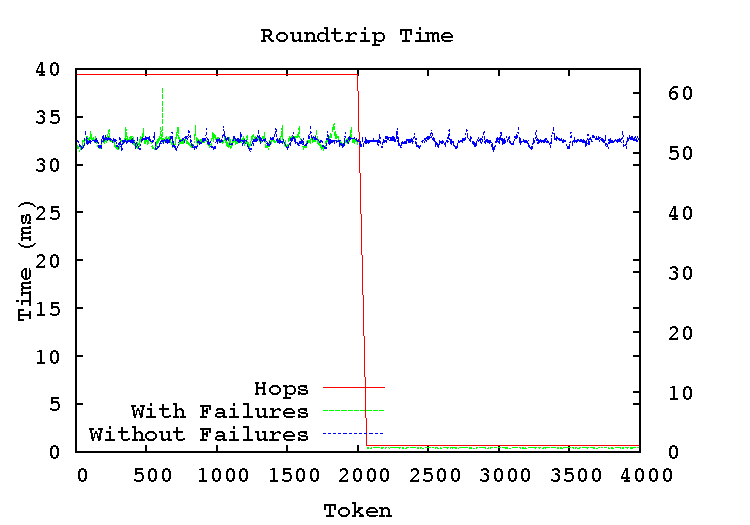
\includegraphics[scale=0.48]{critical.pdf}\label{fig:critical}}
  \caption{Many Processes failing together}\label{fig:many}
\end{figure}
	% Kill 1/2 in middle
Figure~\ref{fig:major} introduces much larger failures at a time. In
this test, half of the processes fail all at once at the midpoint of
the run. While it takes the runtime some time to discover all of the
failures, as illustrated by the larger number of lost tokens, it does
eventually recover from the losses and any tokens that were not on one
of the failed processes at the time of the failure continue around the
ring until rank 0 receives them again.

	% Kill p - 2 in middle
Figure~\ref{fig:critical} introduces a critical failure. In this test,
all but two processes are killed at the same time at the midpoint of
the run. Again, the runtime requires a discovery period before
stabilizing, but it is able to recover and continue delivering the
remaining tokens back to rank 0. Figures~\ref{fig:major}
and~\ref{fig:critical} are encouraging as they show that the runtime
can withstand any number of failures at any time. This implementation
can withstand concurrent or consecutive failures without requiring any
minimal ``cooling off'' period between failures.

\begin{figure}[t]
  \centering
  \subfloat[\small Detection Time for Failures]{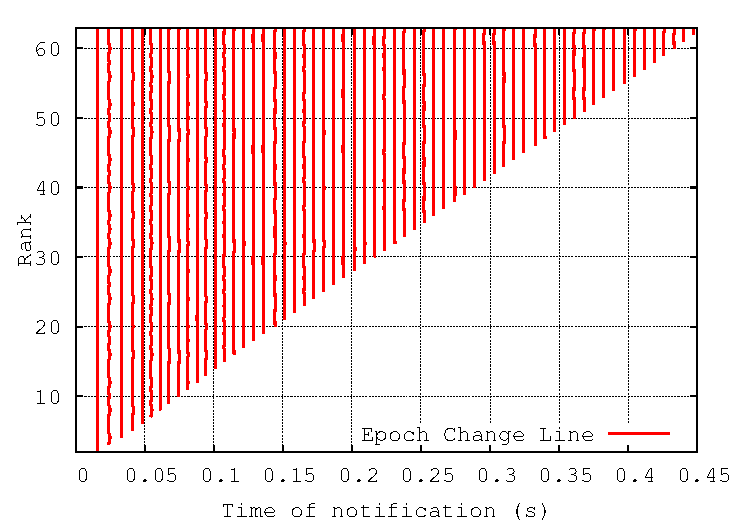
\includegraphics[scale=0.48]{epochs-lines.pdf}\label{fig:detection}}
  \subfloat[\small Overhead Introduced by Changes]{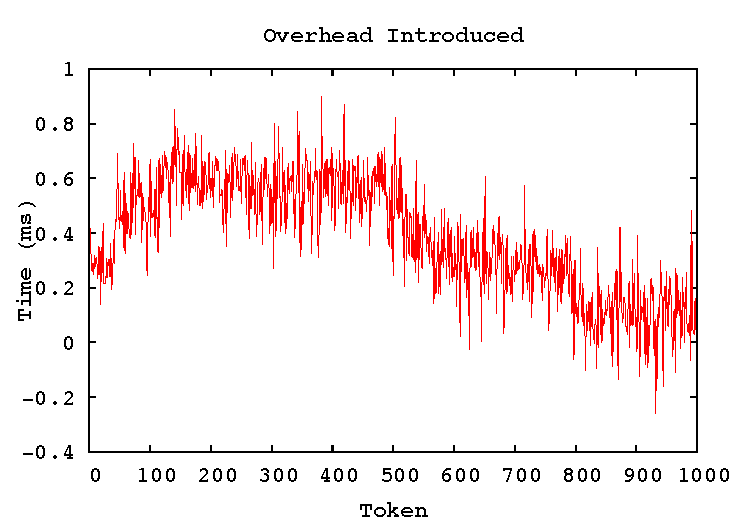
\includegraphics[scale=0.48]{overhead.pdf}\label{fig:overhead}}
  \caption{Overheads of the Resilient Runtime}\label{fig:overheads}
\end{figure}
	% Detection Time
Figure~\ref{fig:detection} shows the detection and notification time
for each failure. It uses the same case as figure~\ref{fig:onebyone} where
failures occur evenly throughout the lifetime of the application. Each
line represents the detection time of each epoch among all the ranks,
collected using the ad-hoc fault handler. To reduce the effect of
clock drift, the time is measured from the beginning of the local
application rather than attempting to synchronize with a single value
from rank 0. When the line is very straight, it demonstrates that the
latency of detection and notification for the failure is relatively low
among all the remaining process. This figure shows that the detection
time for the all processes is very tight, demonstrating that all
processes can maintain a consistent view of the current epoch.

	% Overhead
Figure~\ref{fig:overhead} shows the overhead that was introduced by
modifying the \ompi source code. It compares the runtime of a
fault-free case using both our implementation of the \ompi runtime,
and the revision 24614 of the \ompi trunk. The overhead was measured on a
local 8 node development cluster with minimal system noise to
eliminate outside effects on the data. We subtract the round trip time
for each token in the resilient version of \ompi from the same test
using the trunk version of \ompi. The results show that the changes
made to the code actually had little impact on performance in the
fault-free case. Variations can be explained by the network jitter
and the small increase in the header size of the messages due to the
epoch algorithm.

\section{Conclusion and Future Work}
\label{sect:conclusion}

This paper has demonstrated a runtime system that is able to quickly
detect and recover from multiple process failures. The runtime stabilizes its
internal accounting and passes failures on to an application layer
through callback functions to be invoked following a process failure
notification. Experiments, based on an ad-hoc application, have
demonstrated that the runtime is able to tolerate an arbitrary number
of failures while still providing its basic services and adding
fault-related services.

This demonstrates the feasibility of such a runtime, and the fact that
resilience can be achieved based on series of basic building blocks
that will allow developers who wish to implement a fault tolerant MPI
to easily add their own MPI level fault tolerant capabilities on top
of this runtime.  In the near future, \ompi will be modified to
implement the fault handler ``\texttt{MPI\_ERRORS\_RETURN}'', or other
user-level handler, using these features.


% Future Work
As a further goal, we plan to use this runtime layer to implement
anticipated changes to MPI 3 including run-through stabilization. More
changes could be implemented at the runtime level including a method
for process recovery to give applications more options in their
reactions to faults. With recovery, applications could choose either
to ignore failed processes or create new processes to replace the
failed ones. This introduces a new set of interesting problems at the
runtime layer, such as the restoration of processes to routing layers,
and allows for new methods of recovery such as uncoordinated
rollback. At the MPI layer, restoring processes becomes even more
complex and requires that the MPI processes perform appropriate steps
to recover it failed neighbors. This work continues in the MPI Forum
and will hopefully be adopted soon.

\bibliographystyle{splncs03}
\bibliography{papers}

\end{document}
